\documentclass[spanish, mexico]{beamer}

\usepackage{graphicx}
\usepackage{amsmath}
\usepackage{amsfonts}
\usepackage{amssymb}
\usepackage[utf8]{inputenc}
\usepackage[spanish, mexico]{babel}

\usetheme{Warsaw}



\title[Diffie-Hellman key exchange, ¿Cómo y porqué funciona?]{Diffie-Hellman key exchange} 

\author{Miguel A. Gomez B.}
\institute[FUKL]
{
	Fundación Universitaria Konrad Lorenz\\ 
	\medskip 
	\textit{miguela.gomezb@konradlorenz.edu.co}
}
\date{12 de noviembre de 2019}

\begin{document}
	\begin{frame}
	\titlepage 
	\end{frame}

	\begin{frame}
		\frametitle{Introducción}
		\framesubtitle{¿Criptografía y criptoanálisis?}
		\begin{center}
			\textit{Cripto} + \textit{Grafía} = 'Secreto escrito' 
		\end{center}
		La criptografía es la parte de la criptología(estudio de lo oculto) que trata del diseño e implementación de sistemas secretos \cite{Tnumeros2004}\\~\\
		El criptoanálisis es la parte de la criptología consiste en el estudio de los métodos para decifrar sistemas criptográficos.
	\end{frame}

	\begin{frame}
		\frametitle{Introducción}
		\framesubtitle{Cifrado y Descifrado}
		El \textit{codificador}, es el algoritmo mediante el cual se transforma un texto plano en un texto cifrado, algunos de ellos utilizan una \textit{llave de cifrado}, algunos muy conocidos son blowfish, 3DES, AES, entre otros.\\~\\
		El proceso mediante el cual se convierte el texto plano en texto cifrado, se llama \textit{encripción} o \textit{cifrado}.\\~\\
		El proceso inverso mediante el cual a partir de un texto cifrado se obtiene un texto plano se llama \textit{desencriptación} o \textit{desciframiento}.
	\end{frame}

	\begin{frame}
		\frametitle{Cifrado en la antiguedad}
		\framesubtitle{Un poco de historia}
		Se utilizaron mucho antes de la llegada de los computadores. Como Julio César y Cifrado César.\\~\\
		El cifrado César se llevaba a cabo una operación que consistía en reemplazar cada letra del alfabeto por la letra que se encontraba tres posiciomes adelante.
	\end{frame}

	\begin{frame}
		\frametitle{Cifrado en la antiguedad}
		\framesubtitle{Un poco de historia}
		\begin{table}[]
			\centering
			\resizebox{\textwidth}{!}{%
			\begin{tabular}{| l | l | l | l | l | l | l | l | l | l | l | l | l | l | l | l | l | l | l | l | l | l | l | l | l | l | l |}
				\hline
				A & B & C & D & E & F & G & H & I & J & K & L & M & N & Ñ & O & P & Q & R & S & T & U & V & W & X & Y & Z\\
				\hline
				0 & 1 & 2 & 3 & 4 & 5 & 6 & 7 & 8 & 9 & 10 & 11 & 12 & 13 & 14 & 15 & 16 & 17 & 18 & 19 & 20 & 21 & 22 & 23 & 24 & 25 & 26\\
				\hline
			\end{tabular}%
			}
		\end{table}
		\begin{example}[]
			Cifre el texto 'SECRET' con cifrado César de 3 posiciones.
		\end{example}
		\begin{solution}[]
			Construímos una correspondencia con los valores de la tabla, así: $S = 19, E = 4, C = 2, R = 18, T = 20$ y sumamos tres a cada uno de los valores y ubicamos su correspondencia en la tabla nuevamente. $19 + 3 = 22 = V, 4 + 3 = 7 = H, 2 + 3 = 5 = F, 18 + 3 = 21 = U, 20 + 3 = 23 = W$. de modo que al cifrar la palabra 'SECRETO' obtenemos 'VHFUHW'.
		\end{solution}
	\end{frame}

	\begin{frame}
		\frametitle{Cifrado César}
		\framesubtitle{Es una construcción de módulos}
		\begin{table}[]
			\centering
			\resizebox{\textwidth}{!}{%
				\begin{tabular}{| l | l | l | l | l | l | l | l | l | l | l | l | l | l | l | l | l | l | l | l | l | l | l | l | l | l | l |}
					\hline
					A & B & C & D & E & F & G & H & I & J & K & L & M & N & Ñ & O & P & Q & R & S & T & U & V & W & X & Y & Z\\
					\hline
					0 & 1 & 2 & 3 & 4 & 5 & 6 & 7 & 8 & 9 & 10 & 11 & 12 & 13 & 14 & 15 & 16 & 17 & 18 & 19 & 20 & 21 & 22 & 23 & 24 & 25 & 26\\
					\hline
				\end{tabular}%
			}
		\end{table}
		Si representamos por $P$ el equivalente numérico una de las letras del texto plano y por $C$ su valor al ser cifrado, tenemos que con el cifrado César se deriva la congruencia:
		$$C \equiv P + 3 \pmod{27}$$
	\end{frame}
	
	\begin{frame}
		\frametitle{Cifrado César}
		\framesubtitle{Es una construcción de módulos}
		\begin{center}
		    Entren a www.menti.com con el código 45 83 30 
		\end{center}
	\end{frame}
	
	\begin{frame}
		\frametitle{Cifrado César}
		\framesubtitle{Es una construcción de módulos}
		Teniendo en cuenta lo anterior \textbf{¿Cuál es la congruencia que corresponde al paso de decifrado?}\\~\\
		A) $C \equiv P + 3 \pmod{27}$\\~\\
		B) $P \equiv C + 3 \pmod{27}$\\~\\
		C) $P \equiv C - 3 \pmod{27}$
	\end{frame}

	\begin{frame}
		\frametitle{Cifrado César}
		\framesubtitle{Es una construcción de módulos}
		\begin{table}[]
			\centering
			\resizebox{\textwidth}{!}{%
				\begin{tabular}{| l | l | l | l | l | l | l | l | l | l | l | l | l | l | l | l | l | l | l | l | l | l | l | l | l | l | l |}
					\hline
					A & B & C & D & E & F & G & H & I & J & K & L & M & N & Ñ & O & P & Q & R & S & T & U & V & W & X & Y & Z\\
					\hline
					0 & 1 & 2 & 3 & 4 & 5 & 6 & 7 & 8 & 9 & 10 & 11 & 12 & 13 & 14 & 15 & 16 & 17 & 18 & 19 & 20 & 21 & 22 & 23 & 24 & 25 & 26\\
					\hline
				\end{tabular}%
			}
		\end{table}
		Si representamos por $P$ el equivalente numérico una de las letras del texto plano y por $C$ su valor al ser cifrado, tenemos que con el cifrado César se deriva la congruencia:
		$$C \equiv P + 3 \pmod{27}$$
		Y por consiguiente la congruencia para descifrar el texto será
		$$P \equiv C - 3 \pmod{27}$$ 
	\end{frame}

	\begin{frame}
		\frametitle{Cifrado César}
		\framesubtitle{Es un tipo cifrado}
		El cifrado César es un caso especial de algoritmos de encripción y se les conoce como \textit{translación}, vemos que el cifrado César es de la forma:
		
		$$C \equiv P + k \pmod{27}$$
		con $0 \leq k \leq 26$. A este tipo de cifrados se les conoce en una clasificación más amplia como \textit{transformaciones}. Existen otro tipo de cifrados por sustitución que son más efectivos, uno de los más conocidos es el de Vigenère.
	\end{frame}

	\begin{frame}
		\frametitle{Cifrado en la antiguedad}
		\framesubtitle{Cifrado de Vigenère}
		El elemento principal de este tipo de cifrado es la tabla de Vigenère:
		\begin{table}[]
			\centering
			\resizebox{250pt}{!}{%
			\begin{tabular}{| l | l | l | l | l | l | l | l | l | l | l | l | l | l | l | l | l | l | l | l | l | l | l | l | l | l | l | l |}
				\hline
				& A & B & C & D & E & F & G & H & I & J & K & L & M & N & Ñ & O & P & Q & R & S & T & U & V & W & X & Y & Z\\
				\hline
				B & B & C & D & E & F & G & H & I & J & K & L & M & N & Ñ & O & P & Q & R & S & T & U & V & W & X & Y & Z & A\\
				\hline
				C & C & D & E & F & G & H & I & J & K & L & M & N & Ñ & O & P & Q & R & S & T & U & V & W & X & Y & Z & A & B\\
				\hline
				D & D & E & F & G & H & I & J & K & L & M & N & Ñ & O & P & Q & R & S & T & U & V & W & X & Y & Z & A & B & C\\
				\hline
				E & E & F & G & H & I & J & K & L & M & N & Ñ & O & P & Q & R & S & T & U & V & W & X & Y & Z & A & B & C & D\\
				\hline
				F & F & G & H & I & J & K & L & M & N & Ñ & O & P & Q & R & S & T & U & V & W & X & Y & Z & A & B & C & D & E\\
				\hline
				G & G & H & I & J & K & L & M & N & Ñ & O & P & Q & R & S & T & U & V & W & X & Y & Z & A & B & C & D & E & F\\
				\hline
				H & H & I & J & K & L & M & N & Ñ & O & P & Q & R & S & T & U & V & W & X & Y & Z & A & B & C & D & E & F & G\\
				\hline
				I & I & J & K & L & M & N & Ñ & O & P & Q & R & S & T & U & V & W & X & Y & Z & A & B & C & D & E & F & G & H\\
				\hline
				J & J & K & L & M & N & Ñ & O & P & Q & R & S & T & U & V & W & X & Y & Z & A & B & C & D & E & F & G & H & I\\
				\hline
				K & K & L & M & N & Ñ & O & P & Q & R & S & T & U & V & W & X & Y & Z & A & B & C & D & E & F & G & H & I & J\\
				\hline
				L & L & M & N & Ñ & O & P & Q & R & S & T & U & V & W & X & Y & Z & A & B & C & D & E & F & G & H & I & J & K\\
				\hline					
				M & M & N & Ñ & O & P & Q & R & S & T & U & V & W & X & Y & Z & A & B & C & D & E & F & G & H & I & J & K & L\\
				\hline
				N & N & Ñ & O & P & Q & R & S & T & U & V & W & X & Y & Z & A & B & C & D & E & F & G & H & I & J & K & L & M\\
				\hline
				Ñ & Ñ & O & P & Q & R & S & T & U & V & W & X & Y & Z & A & B & C & D & E & F & G & H & I & J & K & L & M & N\\
				\hline
				O & O & P & Q & R & S & T & U & V & W & X & Y & Z & A & B & C & D & E & F & G & H & I & J & K & L & M & N & Ñ\\
				\hline
				P & P & Q & R & S & T & U & V & W & X & Y & Z & A & B & C & D & E & F & G & H & I & J & K & L & M & N & Ñ & O\\
				\hline
				Q & Q & R & S & T & U & V & W & X & Y & Z & A & B & C & D & E & F & G & H & I & J & K & L & M & N & Ñ & O & P\\
				\hline
				R & R & S & T & U & V & W & X & Y & Z & A & B & C & D & E & F & G & H & I & J & K & L & M & N & Ñ & O & P & Q\\
				\hline
				S & S & T & U & V & W & X & Y & Z & A & B & C & D & E & F & G & H & I & J & K & L & M & N & Ñ & O & P & Q & R\\
				\hline
				T & T & U & V & W & X & Y & Z & A & B & C & D & E & F & G & H & I & J & K & L & M & N & Ñ & O & P & Q & R & S\\
				\hline
				U & U & V & W & X & Y & Z & A & B & C & D & E & F & G & H & I & J & K & L & M & N & Ñ & O & P & Q & R & S & T\\
				\hline
				V & V & W & X & Y & Z & A & B & C & D & E & F & G & H & I & J & K & L & M & N & Ñ & O & P & Q & R & S & T & U\\
				\hline
				W & W & X & Y & Z & A & B & C & D & E & F & G & H & I & J & K & L & M & N & Ñ & O & P & Q & R & S & T & U & V\\
				\hline					
				X & X & Y & Z & A & B & C & D & E & F & G & H & I & J & K & L & M & N & Ñ & O & P & Q & R & S & T & U & V & W\\
				\hline					
				Y & Y & Z & A & B & C & D & E & F & G & H & I & J & K & L & M & N & Ñ & O & P & Q & R & S & T & U & V & W & X\\
				\hline					
				Z & Z & A & B & C & D & E & F & G & H & I & J & K & L & M & N & Ñ & O & P & Q & R & S & T & U & V & W & X & Y\\
				\hline										
			\end{tabular}%
		}
		\end{table}
	\end{frame}

	\begin{frame}
		\frametitle{Cifrado en la antiguedad}
		\framesubtitle{Cifrado de Vigenère}
		En este cifrado, se elige una palabra clave y se organizan cada una de las letras del mensaje en bloques del tamaño de la palabra clave y se realiza una correspondencia con las letras de palabra clave, posteriormente se ubica en el alfabeto de la letra palabra clave y se busca la correspondencia con la letra del texto original.
		\begin{example}
			Utilizando la palabra clave 'SECRET' y la tabla de Vigenère encripte el mensaje:
			\begin{center}
				El hogar es donde está el corazón.
			\end{center}
		\end{example}
	\end{frame}
	\begin{frame}
		\frametitle{Cifrado en la antiguedad}
		\framesubtitle{Cifrado de Vigenère}
		\begin{solution}
			la clave tiene un tamaño de 6 letras, de modo que agrupamos el mensaje en bloques de tamaño 6:
			\begin{center}
				SECRET SECRET SECRET SECRET SEC\\
				ELHOGA RESDON DEESTA ELCORA ZON
			\end{center}
			Para la primera letra del mensaje E, observamos que corresponde con la letra S de la palabra clave, de modo que ubicamos la fila que contiene el alfabeto de S, y buscamos la columna de la letra E, vemos que en el alfabeto de S, E corresponde con la letra W, procedemos de manera sucesiva hasta terminar la codificación del mensaje y obtenemos:
			\begin{center}
				WPJFKT JIUUSG VIGJXT WPEFVT RSP
			\end{center}
		\end{solution}
	\end{frame}

	\begin{frame}
		\frametitle{Cifrado en la antiguedad}
		\framesubtitle{Vulnerabilidad}
		Sin embargo, los cifrados por traslación pueden ser decifrados 'fácilmente' mediante un análisis de la frecuencia de las letras. Con el fin de evitar esto, se utiliza el \textit{cifrado por transpocisión} o \textit{Cifrado por permutación}.\\~\\
		En el cifrado por permutación se realizan cambios en la estructura original del mensaje de acuerdo a una convención o clave. Uno muy conocido es el cifrado de transpocisión en columnas.
	\end{frame}

	\begin{frame}
		\frametitle{Cifrado por transpocisión en columnas}
		En este tipo de cifrado, organizamos el mensaje en una matriz y de acuerdo a una convención o una operación sobre la matriz resultante obtenemos el texto cifrado, por ejemplo si tenemos el mensaje 'EL HOGAR ES DONDE ESTA EL CORAZON' en una matriz de 7 columnas, obtenemos:
		
		\begin{table}[]
			\centering
			\resizebox{150pt}{!}{%
				\begin{tabular}{| l | l | l | l | l | l | l |}
					\hline
					E & L & \space & H & O & G & A\\
					\hline
					R & \space & E & S & \space & D & O\\
					\hline
					N & D & E & \space & E & S & T\\
					\hline
					A & \space & E & L & \space & C & O\\
					\hline					
					R & A & Z & O & N & \space & \space\\
					\hline					
				\end{tabular}%
			}
		\end{table}
		Si establecemos la convención de que el mensaje cifrado se obtenga mediante una lectura desde arriba hacia abajo obtenemos:
		\begin{center}
			RANREA D L ZEEE OL SHN E O CSDG OTOA
		\end{center}
	\end{frame}

	\begin{frame}
		\frametitle{Tipos de Cifrado}
		\framesubtitle{Cifrado en bloque}
		En 1929 el matemático Lister Hill desarrolló el cifrado en bloque, este cifrado funciona sobre bloques de $n$ letras y formándolos en bloques de un mismo tamaño.
	\end{frame}
	
	\begin{frame}
		\frametitle{Tipos de Cifrado}
		\framesubtitle{Cifrado en bloque}
		 Si $A = \begin{pmatrix} a & b \\c & d \end{pmatrix}$ es una matriz de tamaño $2 \times 2$ y $P = \begin{pmatrix} x \\ y \end{pmatrix}$ es un vector con componentes en el anillo conmutativo con identidad $R$, definimos el producto $AP$ mediante:
		$$AP = \begin{pmatrix} a & b \\c & d \end{pmatrix} \begin{pmatrix} x \\ y \end{pmatrix} =  \begin{pmatrix} ax + by\\ cx + dy \end{pmatrix}$$
		el producto entre dos matrices de tamaño $2 \times 2$ lo definimos como:
		$$\begin{pmatrix}a & b\\ c & d\end{pmatrix} \begin{pmatrix}x & y\\ z & w\end{pmatrix} = \begin{pmatrix}ax + bz & ay + bw\\ cx + dz & cy + dw\end{pmatrix}$$
	\end{frame}
	
	\begin{frame}
		\frametitle{Tipos de Cifrado}
		\framesubtitle{Cifrado en bloque}
		 La matrix $A$ es \textit{inversible} si existe otra matriz $B$ tal que $AB = BA = I$, donde I es la identidad $I = \begin{pmatrix}1 & 0\\0 & 1\end{pmatrix}$.\\~\\
		 La matriz $A = \begin{pmatrix} a & b\\ c & d\end{pmatrix}$ es inversible si y sólo si su determinante $\det A = D = ad - bc$ es una unidad del anillo. Es decir $D$ es un elemento inversible para la multiplicación en $R$.\\~\\
		 La inversa de $A$, se denota con $A^{-1}$ y está dada por
 		 $$A^{-1} = D^{-1} \begin{pmatrix}D^{-1}d & -D^{-1}b\\-D^{-1}c & D^{-1}a\end{pmatrix} = \begin{pmatrix}d & -b\\-c & a\end{pmatrix}$$
		 donde $D^{-1}$ es el inverso del determinante $D$ en el anillo $R$.
	\end{frame}
	
	\begin{frame}
		\frametitle{Tipos de Cifrado}
		\framesubtitle{Cifrado en bloque}
		 Para cifrar el texto usando el cifrado Hill, lo dividimos en bloques de dos letras, añadiendo si es necesario al final una letra X que que todos los bloques tengan el mismo tamaño y hallamos los vectores correspondientes a cada bloque, les aplicamos la transformación de la forma:
		 $$C \equiv AP \pmod{n}$$
		 tomando los resultados módulo $n$ y el mcd$(\det A, n) = 1$ para obtener los vectores cifrados.
	\end{frame}
	
	\begin{frame}
		\frametitle{Tipos de Cifrado}
		\framesubtitle{Cifrado en bloque}
		 Teniendo en cuenta lo anterior ¿Cuál congruencia corresponde al proceso de descifrado?\\~\\
		 A)$C \equiv AP^{-1} \pmod{n}$\\~\\
		 B)$C^{-1} \equiv AP \pmod{n}$\\~\\
		 C)$C \equiv A^{-1}P \pmod{n}$\\~\\
		 D)$P \equiv A^{-1}C \pmod{n}$\\~\\
	\end{frame}
	
	\begin{frame}
		\frametitle{Tipos de Cifrado}
		\framesubtitle{Cifrado en bloque}
		 Para cifrar el texto usando el cifrado Hill, lo dividimos en bloques de dos letras, añadiendo si es necesario al final una letra X que que todos los bloques tengan el mismo tamaño y hallamos los vectores correspondientes a cada bloque, les aplicamos la transformación de la forma:
		 $$C \equiv AP \pmod{n}$$
		 tomando los resultados módulo $n$ y el mcd$(\det A, n) = 1$ para obtener los vectores cifrados.\\~\\
		 Y por ende la congruencia para descifrar es
		 $$P \equiv A^{-1}C \pmod{n}$$
	\end{frame}
	
	\begin{frame}
		\frametitle{Tipos de Cifrado}
		\framesubtitle{Cifrado en bloque}
		 \begin{example}
		    Utilizando el alfabeto español, cifremos el mensaje 'YA ENTENDI', aplicando la transformación de la forma $C \equiv AP \pmod{27}$ con $A = \begin{pmatrix}2 & 1\\ 6 & 7\end{pmatrix}$
		 \end{example}
		 \begin{solution}
		    dividimos en bloques de longitud 2 y tenemos
		    \begin{center}
		        YA EN TE ND IX
		    \end{center}
		    Añadimos la X para que todos los bloques tengan el mismo tamaño.
		 \end{solution}
	\end{frame}
	
	\begin{frame}
		\frametitle{Tipos de Cifrado}
		\framesubtitle{Cifrado en bloque}
		 \begin{solution}
		    dividimos en bloques de longitud 2 y tenemos
		    \begin{center}
		        YA EN TE ND IX
		    \end{center}
		    Añadimos la X para que todos los bloques tengan el mismo tamaño. Hallamos los vectores correspondientes:
		    $$
		        \begin{pmatrix}25\\0\end{pmatrix} \begin{pmatrix}4\\13\end{pmatrix}
		        \begin{pmatrix}20\\4\end{pmatrix} \begin{pmatrix}13\\3\end{pmatrix}
		        \begin{pmatrix}8\\24\end{pmatrix}
		    $$
		    Y aplicamos la transformación $C \equiv AP \pmod{27}$ y obtenemos.
		 \end{solution}
	\end{frame}
	
	\begin{frame}
		\frametitle{Tipos de Cifrado}
		\framesubtitle{Cifrado en bloque}
		 \begin{solution}
		    Y aplicamos la transformación $C \equiv AP \pmod{27}$ y obtenemos.
		    $
		    \begin{pmatrix}2 & 1\\ 6 & 7\end{pmatrix}
		    \begin{pmatrix}25\\0\end{pmatrix} = \begin{pmatrix}23\\15\end{pmatrix} \pmod{27}
		    $\\~\\
		    $
		    \begin{pmatrix}2 & 1\\ 6 & 7\end{pmatrix}
		    \begin{pmatrix}4\\13\end{pmatrix} = \begin{pmatrix}21\\7\end{pmatrix} \pmod{27}
		    $\\~\\
		    $
		    \begin{pmatrix}2 & 1\\ 6 & 7\end{pmatrix}
		    \begin{pmatrix}20\\4\end{pmatrix} = \begin{pmatrix}17\\13\end{pmatrix} \pmod{27}
		    $\\~\\
		    $
		    \begin{pmatrix}2 & 1\\ 6 & 7\end{pmatrix}
		    \begin{pmatrix}13\\3\end{pmatrix} = \begin{pmatrix}2\\18\end{pmatrix} \pmod{27}
		    $\\~\\
		    $
		    \begin{pmatrix}2 & 1\\ 6 & 7\end{pmatrix}
		    \begin{pmatrix}8\\24\end{pmatrix} = \begin{pmatrix}13\\0\end{pmatrix} \pmod{27}
		    $\\~\\
		    Con los vectores resultantes construímos el mensaje cifrado
		 \end{solution}
	\end{frame}
	
	\begin{frame}
		\frametitle{Tipos de Cifrado}
		\framesubtitle{Cifrado en bloque}
		 \begin{solution}
		    Con los vectores resultantes construímos el mensaje cifrado:
		    \begin{center}
		        WO UH QN CR NA
		    \end{center}
		 \end{solution}
		 \begin{example}
		    Decifremos el texto SÑ RT BÑ IS TJ utilizando la transformación de la forma $C \equiv AP \pmod{27}$ con $A = \begin{pmatrix}4 & 5\\ 3 & 2 \end{pmatrix}$
		 \end{example}
	\end{frame}
	
	\begin{frame}
		\frametitle{Tipos de Cifrado}
		\framesubtitle{Cifrado en bloque}
		\begin{example}
		    Decifremos el texto SÑ RT BÑ IS TJ utilizando la transformación de la forma $C \equiv AP \pmod{27}$ con $A = \begin{pmatrix}4 & 5\\ 3 & 2 \end{pmatrix}$
		 \end{example}
		 \begin{solution}
		    Primero debemos hallar la inversa de $A$ módulo 27.
		    $$\det{A} = 4 \cdot 2 - 5 \cdot 3 = -7 = 20 \pmod{27}$$
		    Ahora debemos hallar el inverso multiplicativo de $20$ en el anillo. Para ello utilizaremos el algoritmo extendido de Euclídes.
		 \end{solution}
	\end{frame}
	
	\begin{frame}
		\frametitle{Tipos de Cifrado}
		 \begin{solution}
		    Para hallar el inverso de $20$ necesitamos solucionar:
		    $$20x \equiv 1 \pmod{27}$$
		    Nótese que mcd$(20, 27) = 1$, y por lo tanto se puede expresar como la combinación lineal:
		    $$1 = 20x + 27y$$
		    Aplicando el algoritmo de euclides obtenemos:\\~\\
		    $27 = 20 + 7$\\~\\
		    $20 = 7(2) + 6$\\~\\
		    $7  = 6(1) + 1$
		 \end{solution}
	\end{frame}
	
	\begin{frame}
		\frametitle{Tipos de Cifrado}
		 \begin{solution}
		    Para hallar el inverso de $20$ necesitamos solucionar:
		    $$20x \equiv 1 \pmod{27}$$
		    Nótese que mcd$(20, 27) = 1$, y por lo tanto se puede expresar como la combinación lineal:
		    $$1 = 20x + 27y$$
		    Aplicando el algoritmo de euclides obtenemos:\\~\\
		    $27 = 20 + 7 \implies 7 = 27 - 20$\\~\\
		    $20 = 7(2) + 6 \implies 6 = 20 - 7(2)$\\~\\
		    $7  = 6(1) + 1 \implies 1 = 7 - 6(1)$
		 \end{solution}
	\end{frame}
	
	\begin{frame}
		\frametitle{Tipos de Cifrado}
		 \begin{solution}
		    $27 = 20 + 7 \implies 7 = 27 - 20$\\~\\
		    $20 = 7(2) + 6 \implies 6 = 20 - 7(2)$\\~\\
		    $7  = 6(1) + 1 \implies 1 = 7 - 6(1)$\\~\\
		    Realizando sustituciones sucesivas en la última ecuación obtenemos:
		    $$1 = 27(3) - 20(4) = 27(3) + 20(-4)$$
		    de modo que $x=-4$, sin embargo ello implica que $23$ también lo es. Por ende:
		    $$A^{-1} = 23 \begin{pmatrix} 2 & -5\\ -3 & 4\end{pmatrix} = \begin{pmatrix} 26 & -115\\ -69 & 92\end{pmatrix} = \begin{pmatrix} 19 & 20\\ 12 & 11\end{pmatrix} \pmod{27}$$
		 \end{solution}
	\end{frame}
	
	\begin{frame}
		\frametitle{Tipos de Cifrado}
		 \begin{solution}
		    con el valor de $A^{-1}$ podemos aplicar la transformación $P \equiv A^{-1}C \pmod{27}$ y obtenemos:\\~\\
		    $
		        \begin{pmatrix}19 &20\\12&11\end{pmatrix}
		        \begin{pmatrix}19\\14\end{pmatrix} = \begin{pmatrix}20\\4\end{pmatrix} \pmod{27}
		    $\\~\\
		    $
		        \begin{pmatrix}19 &20\\12&11\end{pmatrix}
		        \begin{pmatrix}18\\20\end{pmatrix} = \begin{pmatrix}13\\4\end{pmatrix} \pmod{27}
		    $\\~\\
		    $
		        \begin{pmatrix}19 &20\\12&11\end{pmatrix}
		        \begin{pmatrix}1\\14\end{pmatrix} = \begin{pmatrix}2\\4\end{pmatrix} \pmod{27}
		    $\\~\\
		    $
		        \begin{pmatrix}19 &20\\12&11\end{pmatrix}
		        \begin{pmatrix}8\\19\end{pmatrix} = \begin{pmatrix}19\\8\end{pmatrix} \pmod{27}
		    $\\~\\
		    $
		        \begin{pmatrix}19 &20\\12&11\end{pmatrix}
		        \begin{pmatrix}20\\9\end{pmatrix} = \begin{pmatrix}20\\15\end{pmatrix} \pmod{27}
		    $
		 \end{solution}
	\end{frame}
	
	\begin{frame}
		\frametitle{Tipos de Cifrado}
		 \begin{solution}
		    Con los anteriores ubicamos la correspondencia en el alfabeto original y obtenemos el texto: 'TE NECESITO'.\\~\\
		 \end{solution}
		 Una forma más general de cifrar por bloques, es aplicando a los vectores una transformación afín, con la forma:
		 $$C \equiv AP + B \pmod{n}$$
	\end{frame}
	
	\begin{frame}
		\frametitle{Tipos de Cifrado}
		 \textbf{¿Cuál es la operación inversa para descifrar transformaciones de la forma $C \equiv AP + B \pmod{n}$?}\\~\\
		 A) $C \equiv A^{-1}P + B \pmod{n}$\\~\\
		 B) $P \equiv A^{-1}C + A^{-1}B \pmod{n}$\\~\\
		 C) $P \equiv C + A^{-1}B \pmod{n}$\\~\\
	\end{frame}
	
	\begin{frame}
		\frametitle{Tipos de Cifrado}
		 \begin{solution}
		    Con los anteriores ubicamos la correspondencia en el alfabeto original y obtenemos el texto: 'TE NECESITO'.\\~\\
		 \end{solution}
		 Una forma más general de cifrar por bloques, es aplicando a los vectores una transformación afín, con la forma:
		 $$C \equiv AP + B \pmod{n}$$
		 Por consiguiente su inverso será:
		 $$P \equiv A^{-1}C + A^{-1}B \pmod{n}$$
	\end{frame}
	
	\begin{frame}
		\frametitle{Tipos de Cifrado}
		\framesubtitle{Checkpoint}
		 Otros tipos de cifrado...\\~\\
		 Cifrado de flujo, en el cifrado de flujo, cada parte del texto inicial se cifra en base a la llave llave de cifrado, el siguiente bloque se cifra en base al bloque previo.
	\end{frame}
	
	\begin{frame}
		\frametitle{Diffie-Hellman Key Exchange}
		\framesubtitle{Grupo, anillo y Campo}
		\begin{definition} [Grupo]
		    Un Grupo $(G, *)$ es un conjunto $G$ provisto de una operación binaria $*$ que satisface los axiomas:
		    \begin{itemize}
		        \item G-1: La operación $*$ es asociativa, es decir para todo $a,b,c$ en $G$ se tiene que $a*(b*c) = (a*b)*c$.
		        \item G-2: Existe un elemento $e$ en $G$ tal que $e*a = a*e = a$, para todo $a$ en $G$.
		        \item G-3: Para cada $a$ en $G$ existe un elemento $a'$ en $G$ tal que $a*a' = a'*a = e$.
		    \end{itemize}
		\end{definition}
		Observacion: El elemento $e$ se le denomina como la identidad del grupo y al elemento $a'$ se le conoce como el inverso de $a$ respecto a $*$.
	\end{frame}
	
	\begin{frame}
	    \frametitle{Diffie-Hellman Key Exchange}
		\framesubtitle{Grupo, anillo y Campo}
	    \begin{definition} [Grupo Abeliano (o Conmutativo)]
		    Un grupo $G$ se llama abeliano o conmutativo si satisface la condición
		    $$a*b = b*a$$
		    para todo $a$ y $b$ en $G$.
		\end{definition}
	\end{frame}
	
	\begin{frame}
	    \frametitle{Diffie-Hellman Key Exchange}
		\framesubtitle{Grupo, anillo y Campo}
	    \begin{definition} [Anillo]
		    Un anillo $(A,+,\cdot)$ es un conjunto $A$ provisto de dos operaciones $+$ y $\cdot$, llamados adición y multiplicación que satisface los axiomas siguientes.
		    \begin{itemize}
		        \item A-1: (A,+) es un grupo Abeliano.
		        \item A-2: La multiplicación es asociativa.
		        \item A-3: Las dos operaciones están relacionadas por las propiedades distributivas
		        $$a(b+c) = ab + ac$$
		        $$(b + c)a = ba + ca$$
		        para todo $a,b,c$ en $A$.
		    \end{itemize}
		\end{definition}
	\end{frame}
	
	\begin{frame}
	    \frametitle{Diffie-Hellman Key Exchange}
		\framesubtitle{Grupo, anillo y Campo}
	    \begin{definition} [Anillo Conmutativo]
		    Un anillo donde la multiplicación es conmutativa se dice \textit{anillo conmutativo}. Un anillo que tiene una identidad para la multiplicación que se representa usualmente por $1$, es un \textit{anillo con identidad}.
		\end{definition}
		Observación: $(\mathbb{Z}_n, +, \cdot)$ es un anillo con identidad y conmutativo.
	\end{frame}
	
	\begin{frame}
	    \frametitle{Diffie-Hellman Key Exchange}
		\framesubtitle{Grupo, anillo y Campo}
            Intuición: $\mathbb{Z}_6$ es un anillo con identidad y conmutativo.\\~\\
            Recordemos que $\mathbb{Z}_n$ es el conjunto de cocientes módulo $n$ y que $\overline{\rm a}$ es la clase residual módulo $n$, luego para este caso específico
            $$\mathbb{Z}_6 = \{ \overline{\rm 0}, \overline{\rm 1}, \overline{\rm 2}, \overline{\rm 3}, \overline{\rm 4}, \overline{\rm 5} \}$$
        	Ituición de que $(\mathbb{Z}_6, +)$ es un grupo. Tomemos las congruencias $11 \equiv 5 \pmod{6}$ y $28 \equiv 4 \pmod{6}$, sabemos de antemano que $9 \equiv 3 \pmod{6}$, ahora sumemoslas:
        	$$11 + 28 \equiv 9 \pmod{6}$$
        	$39 \equiv 9 \pmod{6}$ y como $9 \equiv 3 \pmod{6}$, entonces $39 \equiv 3 \pmod{6}$ luego pertenece al grupo.
	\end{frame}
	
	\begin{frame}
	    \frametitle{Diffie-Hellman Key Exchange}
		\framesubtitle{Grupo, anillo y Campo}
        Otra forma de verlo sería utilizando la suma de las clases residuales, para ello requerimos de la siguiente definición.
        \begin{definition}
            Sobre $\mathbb{Z}_n$, podemos definir una adición y una multiplicación:
            $$\overline{\rm a} + \overline{\rm b} = \overline{\rm ab}$$
            $$\overline{\rm a}\cdot \overline{\rm b} = \overline{\rm ab}$$
        \end{definition}
        Cómo sabemos las clases residuales para $(11)_6$ y $(28)_6$ son respectivamente $\overline{\rm a}$ y $\overline{\rm b}$, de modo que por la definición anterior
        $$\overline{\rm 5} + \overline{\rm 4} = \overline{\rm 9} = \overline{\rm 3}$$
	\end{frame}
	
	\begin{frame}
	    \frametitle{Diffie-Hellman Key Exchange}
		\framesubtitle{Grupo, anillo y Campo}
		Para los proximos, requerimos de las siguientes propiedades
        \begin{theorem}
            La adición en $\mathbb{Z}_n$ tiene las propiedades siguientes:
            \begin{itemize}
                \item $\overline{\rm a} + (\overline{\rm b} + \overline{\rm c}) = (\overline{\rm a} + \overline{\rm b}) + \overline{\rm c}$
                \item $\overline{\rm a} + \overline{\rm 0} = \overline{\rm 0} + \overline{\rm a} = \overline{\rm a}$
                \item Para cada $\overline{\rm a}$ existe $\overline{\rm x}$ tal que $\overline{\rm a} + \overline{\rm x} = \overline{\rm x} + \overline{\rm a} = \overline{\rm 0}$
                \item $\overline{\rm a} + \overline{\rm b} = \overline{\rm b} + \overline{\rm a}$
            \end{itemize}
        \end{theorem}
        Intuición de que $(\mathbb{Z}_6, + )$ es conmutativo:
            $$\overline{\rm 5} + \overline{\rm 4} = \overline{\rm 5 + 4} = \overline{\rm 4 + 5} = \overline{\rm 9} = \overline{\rm 3}$$
	\end{frame}
	
	\begin{frame}
	    \frametitle{Diffie-Hellman Key Exchange}
		\framesubtitle{Grupo, anillo y Campo}
		Intuición de que $(\mathbb{Z}_6, + )$ es asociativo:
            $$(\overline{\rm 5} + \overline{\rm 4}) + \overline{\rm 3} = \overline{\rm 5 + 4} + \overline{\rm 3} = \overline{\rm 5 + 4 + 3} = \overline{\rm 5} + \overline{\rm 4 + 3} = \overline{\rm 5} + \overline{\rm 7} = \overline{\rm 12} = \overline{\rm 0}$$
        $(\mathbb{Z}_6, +)$ tiene un elemento neutro. $\overline{\rm 0}$ es el elemento neutro:
        $$\overline{\rm 1} + \overline{\rm 0} = \overline{\rm 0 + 1} = \overline{\rm 1}$$
        $(\mathbb{Z}_6, +)$ satisface la propiedad del inverso.
        $$\overline{\rm 1} + \overline{\rm 1}' = \overline{\rm 0} \implies \overline{\rm 1}' = \overline{\rm 5} \implies \overline{\rm 1 + 5} = \overline{\rm 6} = \overline{\rm 0}$$
        Observación $\overline{\rm 0}$ es la identidad de $(\mathbb{Z}_6, +)$, por ende será un grupo abeliano.
	\end{frame}
	
	\begin{frame}
	    \frametitle{Diffie-Hellman Key Exchange}
		\framesubtitle{Grupo, anillo y Campo}
		$(\mathbb{Z}_6, \cdot)$ es asociativa. Intuición,
		$$
    		\overline{\rm 5} \cdot \overline{\rm 1} \cdot \overline{\rm 2} = \overline{\rm 5\cdot 1} \cdot \overline{\rm 2} = \overline{\rm 5 \cdot 1 \cdot 2} = \overline{\rm 5} \cdot \overline{\rm 1 \cdot 2} = \overline{\rm 5} \overline{\rm 2} = \overline{\rm 10} = \overline{\rm 4}
		$$
		$(\mathbb{Z}_6, +, \cdot)$ tiene las dos operaciones relacionadas con la propiedad distributiva. Intuición,
		\begin{align*}
		    \overline{\rm 2} \cdot (\overline{\rm 3} + 5) = \overline{\rm 2} (\overline{\rm 3 + 5}) = \overline{\rm 2(3+5)} &= \overline{\rm 2\cdot 3 + 2 \cdot 5}\\
		    &= \overline{\rm 3\cdot 2} + \overline{\rm 5 \cdot 2}\\
		    &= \overline{\rm 6} + \overline{\rm 10}\\
		    &= \overline{\rm 16}\\
		    &= \overline{\rm 4}
		\end{align*}
	\end{frame}
	
	\begin{frame}
	    \frametitle{Diffie-Hellman Key Exchange}
		\framesubtitle{Grupo, anillo y Campo}
	    $(\mathbb{Z}_6, +, \cdot)$ es un anillo conmutativo. Intuición:
	    $$\overline{\rm 2} \cdot \overline{\rm 5} = \overline{\rm 2 \cdot 5} = \overline{\rm 5 \cdot 2} = \overline{\rm 5} \cdot \overline{\rm 2}$$
	    $(\mathbb{Z}_6, +, \cdot)$ es un anillo con identidad:
	    $\overline{\rm 1} \cdot \overline{5} = \overline{1\cdot5} = \overline{5}$
	    \begin{definition}[Anillo de enteros módulo $n$]
	    Si $(\mathbb{Z}_n, +, \cdot)$ Es un anillo conmutativo con identidad. La identidad e este anillo es precisamente $\overline{\rm 1}$. Este anillo se llama el \textit{anillo de los enteros}
	    \end{definition}
	    \begin{definition}[Divisores de cero]
	    Decimos que un anillo $(A, +, \cdot)$ tiene \textit{divisores de cero} si existen $a,b \in A$ distintos de cero, pero tales que $ab = 0$
	    \end{definition}
	    Intuición: $(\mathbb{Z}_6, +, \cdot)$ tiene divisores de cero por que:
	    $$\overline{\rm 2} \cdot \overline{\rm 3} = \overline{\rm 6} = \overline{\rm 0}$$
	\end{frame}
	
	\begin{frame}
	    \frametitle{Diffie-Hellman Key Exchange}
		\framesubtitle{Grupo, anillo y Campo}
	    Observación: $(\mathbb{Z}_6, +, \cdot)$ no cumple la ley cancelativa para la multiplicación ya que tenemos que:
	    $$\overline{\rm 3} \cdot \overline{\rm 2} = \overline{\rm 3} \cdot \overline{\rm 4}$$
	    pero $\overline{\rm 2} \neq \overline{\rm 4}$. Esto es consecuencia del siguiente teorema.
	    \begin{theorem}
	        Un anillo $A$ satisface la ley cancelativa para la multiplicación a izquierda y derecha, si y sólo si $A$ no tiene divisores de cero.
	    \end{theorem}
	\end{frame}
	
	\begin{frame}
	    \frametitle{Diffie-Hellman Key Exchange}
		\framesubtitle{Grupo, anillo y Campo}
	    \begin{theorem}[A]
	        Un anillo $A$ satisface la ley cancelativa para la multiplicación a izquierda y derecha, si y sólo si $A$ no tiene divisores de cero.
	    \end{theorem}
	    \begin{block}{Demostración}
	        Suponga que $A$ es  un anillo sin divisores de cero. Si  $a,b,c \in A$ con $a \neq 0$ y $ab = ac$ entonces
	        \begin{align*}
	            ab &= ac\\
	            ab - ac &=0\\
	            a(b-c) &=0
	        \end{align*}
	    \end{block}
	\end{frame}
	
	\begin{frame}
	    \frametitle{Diffie-Hellman Key Exchange}
		\framesubtitle{Grupo, anillo y Campo}
	    \begin{block}{Demostración Cont.}
	        como $a \neq 0$ entonces $(b-c) = 0 \implies b = c$ por ende:
	        $$ab = ac$$
	        $$a = a$$
	        De manera análoga se cumple la ley cancelativa a la derecha.\\~\\
	        Suponga ahora que $A$ satisface la ley cancelativa para la multiplicación. Si $ab = 0$ con $a \neq 0$ entonces $ab = a(0)$, por ley cancelativa $b=0$, análogamente se cumple si elegimos $b\neq0$. Luego $A$ no tiene divisores de cero. $\qed$
	    \end{block}
	\end{frame}
	
	\begin{frame}
	    \frametitle{Diffie-Hellman Key Exchange}
		\framesubtitle{Grupo, anillo y Campo}
	    \begin{definition}[Dominio de integridad]
	        Un dominio de integridad es un anillo conmutativo, con identidad y sin divisores de cero.
	    \end{definition}
	    \begin{definition}[Cuerpo]
	        Un cuerpo es un anillo conmutativo con identidad en el cual todo elemento distinto de cero tiene un inverso para la multiplicación.
	    \end{definition}
	    \begin{definition}
	        Los elementos invertibles para la mutiplicación en un anillo con identidad se llaman las unidades del anillo.
	    \end{definition}
	    Observación: En un cuerpo las unidades del anillo son todos los elementos distintos de cero.
	\end{frame}
	
	\begin{frame}
	    \frametitle{Diffie-Hellman Key Exchange}
		\framesubtitle{Grupo, anillo y Campo}
	    \begin{theorem}[D] Todo cuerpo es un dominio de integridad.
	    \end{theorem}
	    \begin{proof}
	        Como un cuerpo es un anillo conmutativo con identidad, por el teorema (A), luego sólo resta demostrar que se cumple la ley cancelativa. Suponga que $a\neq0$ y $ab = ac$.\\~\\
	        $a'$ es el inverso multiplicativo de $a$, es decir $aa' = 1$, multiplicamos por $a'$
	        $$aba' = aca'$$
	        por asociatividad y conmutatividad $(aa')b = c(aa')$ por ende $b = c$.
	    \end{proof}
	\end{frame}
	
	\begin{frame}
	    \frametitle{Diffie-Hellman Key Exchange}
		\framesubtitle{Grupo, anillo y Campo}
	    \begin{theorem}[B]
	        En el anillo $\mathbb{Z}_n$ los divisores de cero son precisamente los elementos $\overline{\rm m} \neq 0$ tales que $m$ y $n$ no son primos relativos.
	    \end{theorem}
	    Intuición
	    Precisamente los elementos $\overline{\rm m} \neq 0$ tales que no son primos relativos en $\mathbb{Z}_6$son: $\overline{\rm 2}, \overline{\rm 3} \text{ y } \overline{\rm 4}$, ahora observese lo siguiente:
	    $$
	        \text{mcd}(6, 2) = 2 \text{ luego, } \overline{\rm 2} \overline{\rm (6/2)} = \overline{\rm 2(6/2)} = \overline{\rm 6}\overline{\rm (2/2)} = \overline{\rm 6} \overline{\rm 1} = \overline{\rm 6} = \overline{\rm 0}
	    $$
	    $$
	        \text{mcd}(6, 3) = 3 \text{ luego, } \overline{\rm 3} \overline{\rm (6/3)} = \overline{\rm 3(6/3)} = \overline{\rm 6}\overline{\rm (3/3)} = \overline{\rm 3} \overline{\rm 1} = \overline{\rm 6} = \overline{\rm 0}
	    $$
	    $$
	        \text{mcd}(6, 4) = 2 \text{ luego, } \overline{\rm 4} \overline{\rm (6/2)} = \overline{\rm 4(6/2)} = \overline{\rm 6}\overline{\rm (4/2)} = \overline{\rm 6} \overline{\rm 2} = \overline{\rm 12} = \overline{\rm 0}
	    $$
	\end{frame}
	
	\begin{frame}
	    \frametitle{Diffie-Hellman Key Exchange}
		\framesubtitle{Grupo, anillo y Campo}
	    \begin{proof}
	        Sea $\overline{\rm m} \neq \overline{\rm 0}$ tales que $m$ y $n$ no son primos relativos. Entonces mcd$(m, n) = d, d > 1$, tenemos
	        $$\overline{\rm m} \overline{\rm (n/d)} = \overline{\rm m(n/d)} = \overline{\rm n(m/d)} = \overline{\rm 0}$$
	        Como $\overline{\rm m} \neq \overline{\rm 0}$ y $\overline{\rm m} \neq \overline{\rm (n/d)}$, pues $d > 1$, se concluye que $\overline{\rm m}$ es un divisor de cero en $\mathbb{Z}_n$. Supongamos ahora que $\overline{\rm m} \in \mathbb{Z}_n$ con $m$ y $n$ primos relativos. Si $\overline{\rm m} \overline{\rm k} = \overline{\rm 0}$ entonces $\overline{\rm mk} =$, luego $mk \equiv 0 \pmod{n}$, luego $n|mk$ y como mcd$(n,m) = 1$ entonces $n|k$ y así $k \equiv 0 \pmod{n}$ o sea $\overline{\rm k} = \overline{\rm 0}$. Por lo tanto $\overline{\rm m}$ no es un divisor de cero. 
	    \end{proof}
	\end{frame}
	
	\begin{frame}
	    \frametitle{Diffie-Hellman Key Exchange}
		\framesubtitle{Grupo, anillo y Campo}
	    \begin{corollary}
	        $\mathbb{Z}_n$ es un dominio de integridad si y sólo si n es un número primo.
	    \end{corollary}
	    \begin{proof}
	        Vamos primero que si $n$ no es primo entonces $\mathbb{Z}_n$ no es un dominio de integridad. Supongamos que $n=ab$ con $1<a<n$ y $1<b<n$, entonces
	        $$\overline{\rm a} \overline{\rm b} = \overline{\rm ab} = \overline{\rm n} = \overline{\rm 0}$$
	        con $a\neq0$ y $b\neq0$. Luego $\mathbb{Z}_n$ tiene divisores de cero y no es dominio de integridad. Suponemos ahora que $n$ es primo, como $n$ es primo relativo con cada uno de los enteros $1,2,\dots, n-1$ por el teorema B, $\mathbb{Z}_n$ no tiene divisores de cero y en consecuencia es un dominio de integridad.
	    \end{proof}
	\end{frame}
	
	\begin{frame}
	    \frametitle{Diffie-Hellman Key Exchange}
		\framesubtitle{Grupo, anillo y Campo}
	    \begin{theorem}
	        $\mathbb{Z}_n$ es un cuerpo si y sólo si $n$ es un número primo.
	    \end{theorem}
	    \begin{block}{Demostración.}
	        Si $n$ no es primo, por el corolario anterior $\mathbb{Z}_n$ no es dominio de integridad y por el teorema D, $\mathbb{Z}_n$ no es un campo. Supongamos ahora que $n$ es un número primo, para probar que $\mathbb{Z}_n$ es un campo, es suficiente probar que todo elemento distinto de cero en $\mathbb{Z}_n$ es una unidad. Para ello, sea $\overline{\rm m} \in \mathbb{Z}_n$ con $0<m<n$. Como $m$ y $n$ son primos relativos, por el lema de bezout existen enteros $r$ y $s$ que satisfacen
	        $$mr + ns = 1$$
	        por lo tanto
	        $$\overline{\rm m}\overline{\rm r} + \overline{\rm n} \overline{\rm s} = \overline{\rm 1}$$
	    \end{block}
	\end{frame}
	
	\begin{frame}
	    \frametitle{Diffie-Hellman Key Exchange}
		\framesubtitle{Grupo, anillo y Campo}
	    \begin{block}{Demostración. Cont.}
	        como $\overline{\rm n} = \overline{\rm 0}$, nos queda
	        $$\overline{\rm m}\overline{\rm r} = 1$$
	        de esta forma vemos que $\overline{\rm r}$ es el inverso multiplicativo de $\overline{\rm m}$ y $\mathbb{Z}_n$ es un cuerpo como se quería demostrar. $\qed$
	    \end{block}
	\end{frame}
	
	\begin{frame}
		\frametitle{La estructura $\mathbb{Z}/p\mathbb{Z}$}
		$\mathbb{Z}/p\mathbb{Z}$: El conjunto de enteros módulo $p$.\\~\\
		 La relevancia de lo anterior implica que si $p$ es un primo entonces $\mathbb{Z}/p\mathbb{Z}$ forma un campo. Básicamente es un conjunto con adición, sustracción, multiplicación  y división (sin el cero) definidas, lo que nos va a permitir construir métodos para dividir enteros sin salirnos del conjunto.
	\end{frame}

	\begin{frame}
		\frametitle{El problema}
		\framesubtitle{¿Porqué aún no es seguro?}
		La fortaleza del sistema depende de que un posible atacante desconozca el algoritmo de cifrado o el la complejidad de encontrar los valores de la llave que permiten decodificar el mensaje
	\end{frame}

	\begin{frame}
		\frametitle{Diffie Hellman Key exchange}
		\framesubtitle{Merkle, Diffie y Hellman}
		Merkle, parece ser la primera persona que disertó acerca del problema y construyó rompecabezas que ilustraban el uso de una técnica con llaves públicas, sin embargo lo descartó debido a que no era práctico computacionalmente.\\~\\
		Whitefield Diffie, se interesa en la criptografía debido que su novia se encontraba investigando cifrados de flujo, reacio a trabajar con la NSA busca expertos en criptografía, hasta que en cierto momento escucha de alguien interesado en las mismas preguntas. En 1976 se publica finalmente el artículo "New Directions in criptography", en donde se explican los detalles de un nuevo mecanismo para compartir las llaves de cifrado.
	\end{frame}

	\begin{frame}
		\frametitle{Diffie-hellman Key exchange}
		\framesubtitle{¿Cómo funciona?}
		Se eligen $g$ y $n$, donde $g$ es un número primo y $n$ es la base, ambos números enteros.\\~\\
		Cada una de las partes elige un número $1<a<n$ y $1<b<n$, que no comparten. La parte que conoce el valor de $a$ calcula $g^{a} \equiv x \pmod{n}$ y la parte que conoce $b$ realiza la misma operación, calcula $$g^{b} \equiv y \pmod{n}$$, ambos intercambian los valores de $x$ y $y$, de modo que ahora cada uno está en capacidad de computar la llave secreta. 
	\end{frame}
	\begin{frame}
	    \frametitle{Diffie-hellman Key exchange}
		\framesubtitle{Ejemplo}
		Tenemos Tres personas, Alice, Bob e Eve, Alice y Bob quieren comunicarse sin que Eve lo note
		\begin{itemize}
		    \item inicialmente eligen $g=7$ y $n=11$.
		    \item Alice elige el número $a=3$, y calcula $g^{a} \pmod{n} = x$ y obtiene $7^{3} \pmod{11} = 2$. $x=2$.
		    \item Bob elige el número $b=6$, y calcula $g^{b} \pmod{n} = y$ y obtiene $7^{6} \pmod{11} = 4$. $y=4$
		    \item Alice comparte $x$ a Bob y éste comparte $y$ a Alice, de modo que Eve, conoce $x,y,g$ y $n$.
		    \item Alice computa la clave secreta $k = y^{a} \pmod{n}$ que es igual a $k_1 = 4^{3} \pmod{11} = 9$.
		    \item Bob realiza lo mismo y computa la clave secreta $k_2 = x^{b} \pmod{n}$ que es igual a $k_2 = 2^{6} \pmod{11} = 9$.
		    \item por lo tanto a partir de este punto ambos comparten una llave que no conoce Eve y por ende no podrá decodificar 'fácilmente' sus mensajes.
		\end{itemize}   
	\end{frame}

	\begin{frame}
		\frametitle{Diffie-Hellman Key Exchange}
		\framesubtitle{¿Porqué funciona?}
		\begin{itemize}
		    \item Por la estructura de cuerpo $\mathbb{Z}/p\mathbb{Z}$. (Y lo anteriormente dicho).
		    \item Por el problema del logaritmo discreto. Que deriva en la dificultad de calcular los valores elegidos por Alice y Bob como llaves secretas.
		    \item En la realidad, los valores de $n$ y $g$ pueden ser de mas de 100 dígitos.
		\end{itemize}
	\end{frame}

	\begin{frame}
		\frametitle{Diffie-Hellman Key Exchange}
		\framesubtitle{El problema del logaritmo discreto}
		Si $a, b$ y $n$ son números reales con $a,b>0$ y $n\geq0$ la función logaritmo base $b$ se caracteriza por:
		$$\log_b{a}=n \Longleftrightarrow a = b^n$$
		En los reales podemos encontrar una respuesta aproximada, sin embargo como todos los valores del algoritmo se construyen en base a la estructura $\mathbb{Z}/p\mathbb{Z}$, implica que la solución debe ser 'exacta', lo cual es un problema muy 'dificil'.
	\end{frame}
	
	\begin{frame}
		\frametitle{Diffie-Hellman Key Exchange}
		\framesubtitle{El problema del logaritmo discreto}
		\begin{center}
		    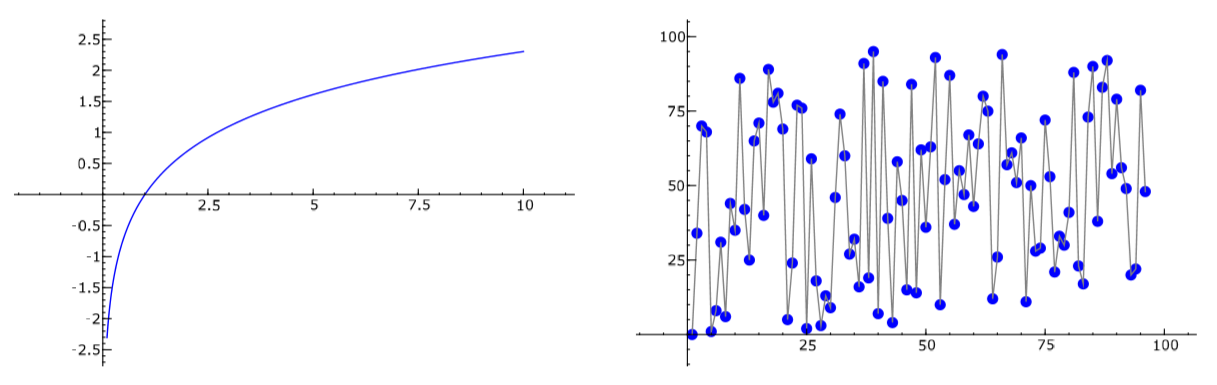
\includegraphics[scale=0.35]{dl.png}
	    \end{center}
	    Tomado de \cite{Stein}. Se comparan el logaritmo en $\mathbb{R}$ y en $\mathbb{Z}$.
	\end{frame}

	\begin{frame}
		\frametitle{Referencias bibliográficas}
		\footnotesize{
		\begin{thebibliography}{1}
			\bibitem[1]{Tnumeros2004} Luis Becerra et. al (2004)
			\newblock Teoría de números para principiantes.
			\newblock p 194-210.
		\end{thebibliography}
		\begin{thebibliography}{2}
			\bibitem[2]{Stein} William Stain (2017)
			\newblock Elementary Number Theory: Primes, Congruences, and secrets.
			\newblock p 49-56.
		\end{thebibliography}
		\begin{thebibliography}{3}
			\bibitem[3]{Holden} Joshua Holden (2017)
			\newblock Mathematics of secrets.
			\newblock p 201-216.
		\end{thebibliography}	
		}
	\end{frame}
\end{document}